\section{Istruzioni all'uso}

\subsection{Landing page}
All'avvio del prodotto verrà visualizzata la landing page, che presenta il logo dell'assistente virtuale e un messaggio di benvenuto. In questa fase, l'utente può scegliere di accedere al sistema.
\begin{figure}[h!]
    \centering
    \includegraphics[width=0.8\textwidth]{./img/landingPage.png}
    \caption{Schermata della landing page}
\end{figure}

\subsection{Pagina di Accesso}
Cliccando sul bottone blu si passerà direttamente alla pagina di accesso, dove l'utente dovrà inserire le proprie credenziali (\textit{username} e \textit{password}) per autenticarsi.
\begin{figure}[h!]
    \centering
    \includegraphics[width=0.8\textwidth]{./img/paginaAccesso.png}
    \caption{Schermata della pagina di accesso}
\end{figure}

\subsection{Pagina di Registrazione}
Nel caso in cui non si possieda un account, è possibile registrarsi dalla pagina di registrazione cliccando sul link presente nella pagina di autenticazione.
Qui l'utente dovrà inserire i campi obbligatori \{ \textit{username; password; email; nome; cognome} \} e volendo opzionalmente può inserire il numero di telefono.
\begin{figure}[h!]
    \centering
    \includegraphics[width=0.8\textwidth]{./img/paginaRegistrazione.png}
    \caption{Schermata della pagina di registrazione}
\end{figure}

\subsection{Schermata iniziale}
Una volta effettuato l'accesso verremo accolti da questa Schermata iniziale composta da 3 elementi, una navbar superiore, una navbar laterale e il contenuto della pagina. Da qui è possibile iniziare una conversazione mettendo il titolo della conversazione e schiacciando il bottone: "inizia la conversazione".
\begin{figure}[h!]
    \centering
    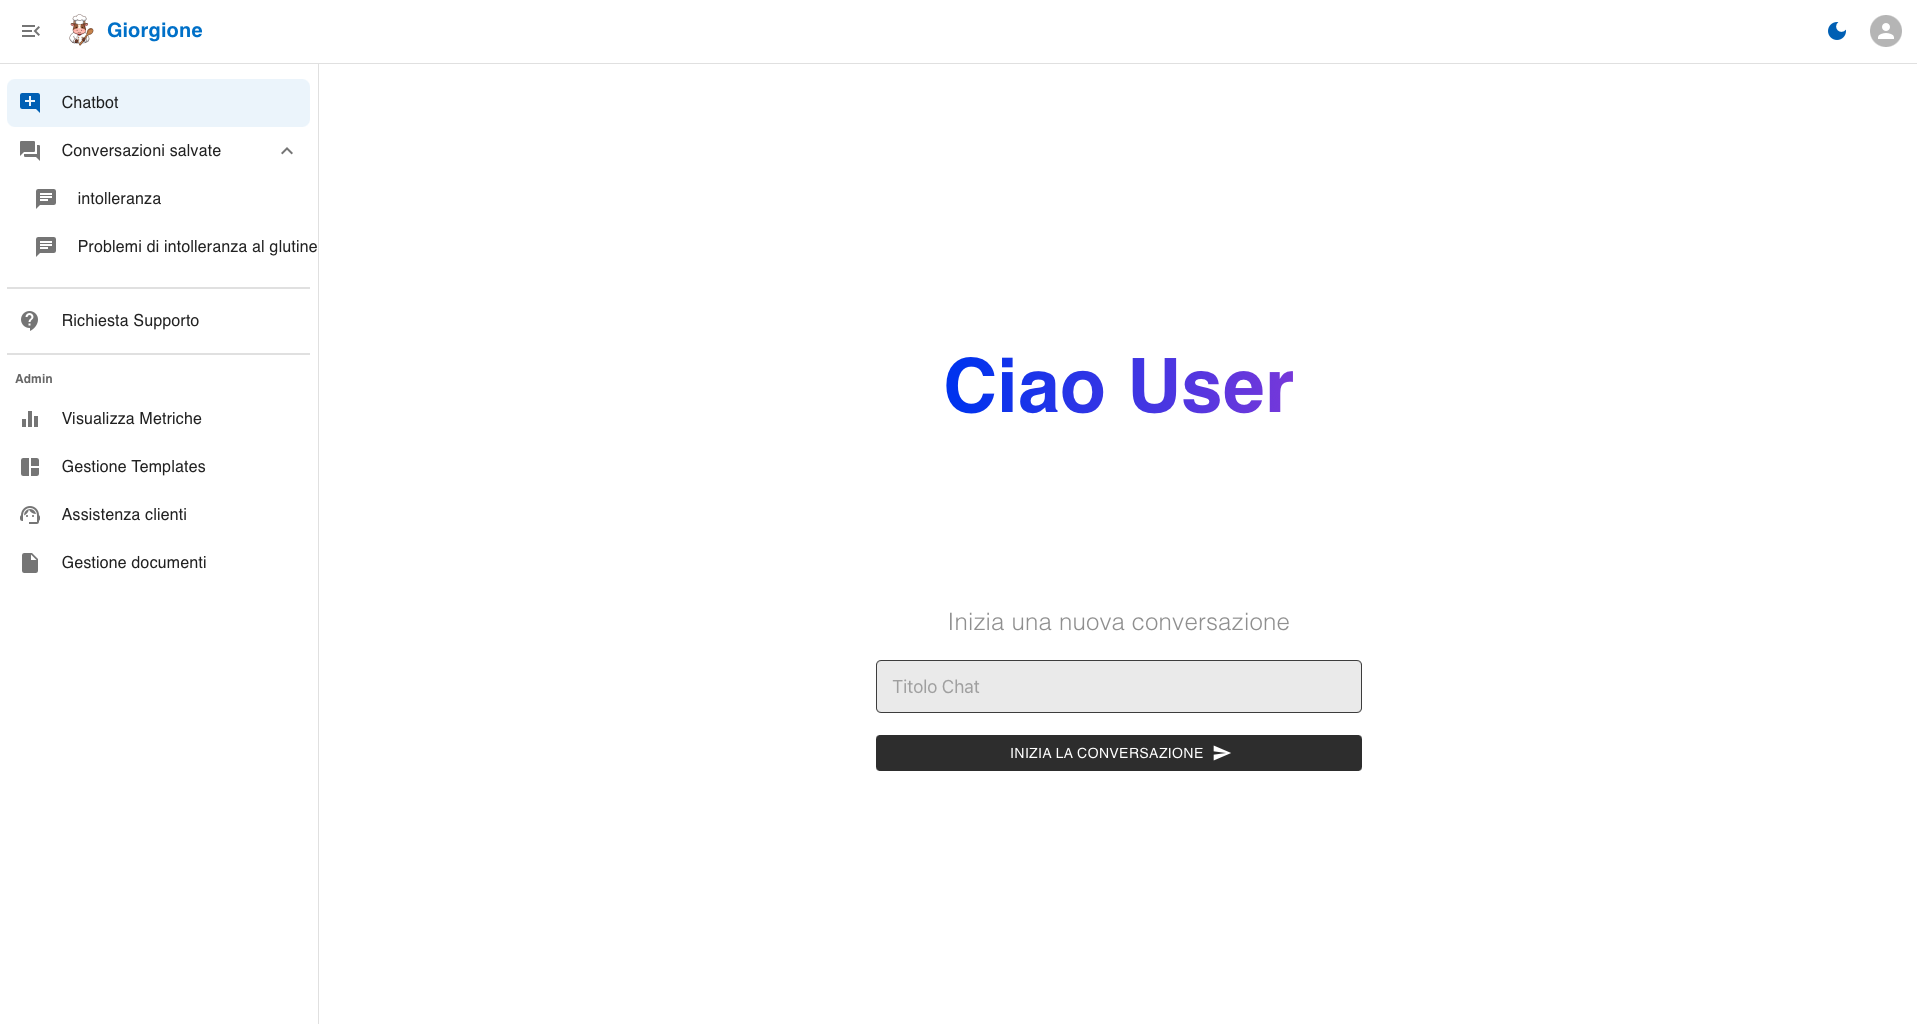
\includegraphics[width=0.8\textwidth]{./img/paginaIniziale.png}
    \caption{Schermata della pagina di registrazione}
\end{figure}

\subsection{Schermata di conversazione}
Una volta creata la conversazione dalla schermata iniziale l'utente può andare nel menù laterale (\textit{nel caso esso sia chiuso si può aprire tramite menù ad hamburger}) e selezionare la voce: "\textit{Conversazioni salvate}" che aprirà un menù a tendina dove l'utente potrà selezionare la conversazione desiderata.
\begin{figure}[h!]
    \centering
    \begin{subfigure}{0.3\textwidth}
        \centering
        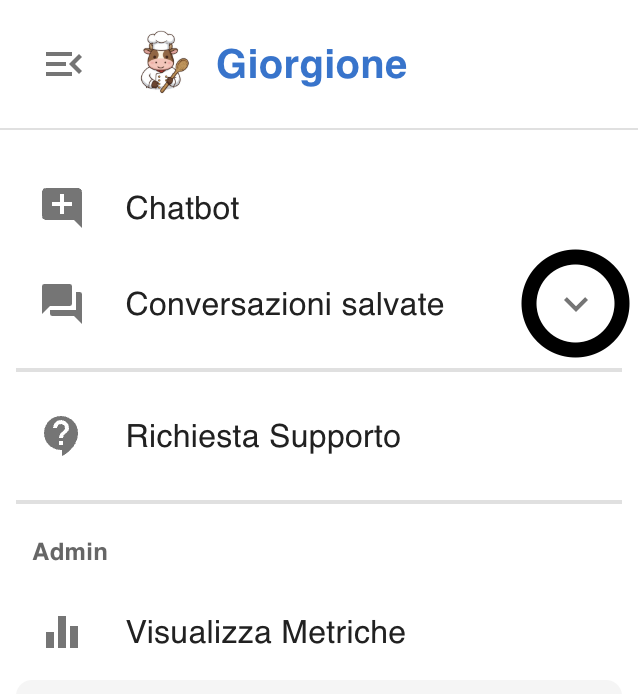
\includegraphics[width=\textwidth]{./img/laterale1.png}
    \end{subfigure}
    \hspace{0.05\textwidth}
    \begin{subfigure}{0.3\textwidth}
        \centering
        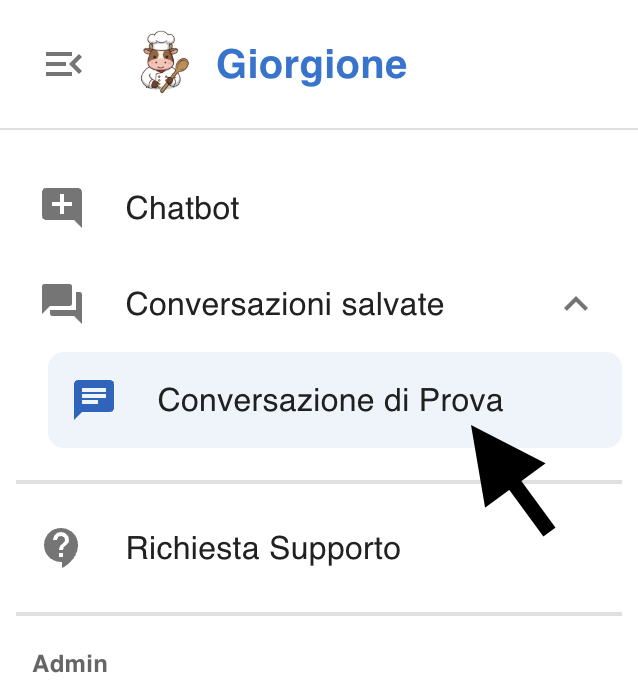
\includegraphics[width=\textwidth]{./img/laterale2.png}
    \end{subfigure}
    \caption{Menù laterale}
\end{figure}
L'utente si trovera quindi di fronte a una schermata composta da diversi elementi:
\begin{figure}[h!]
    \centering
    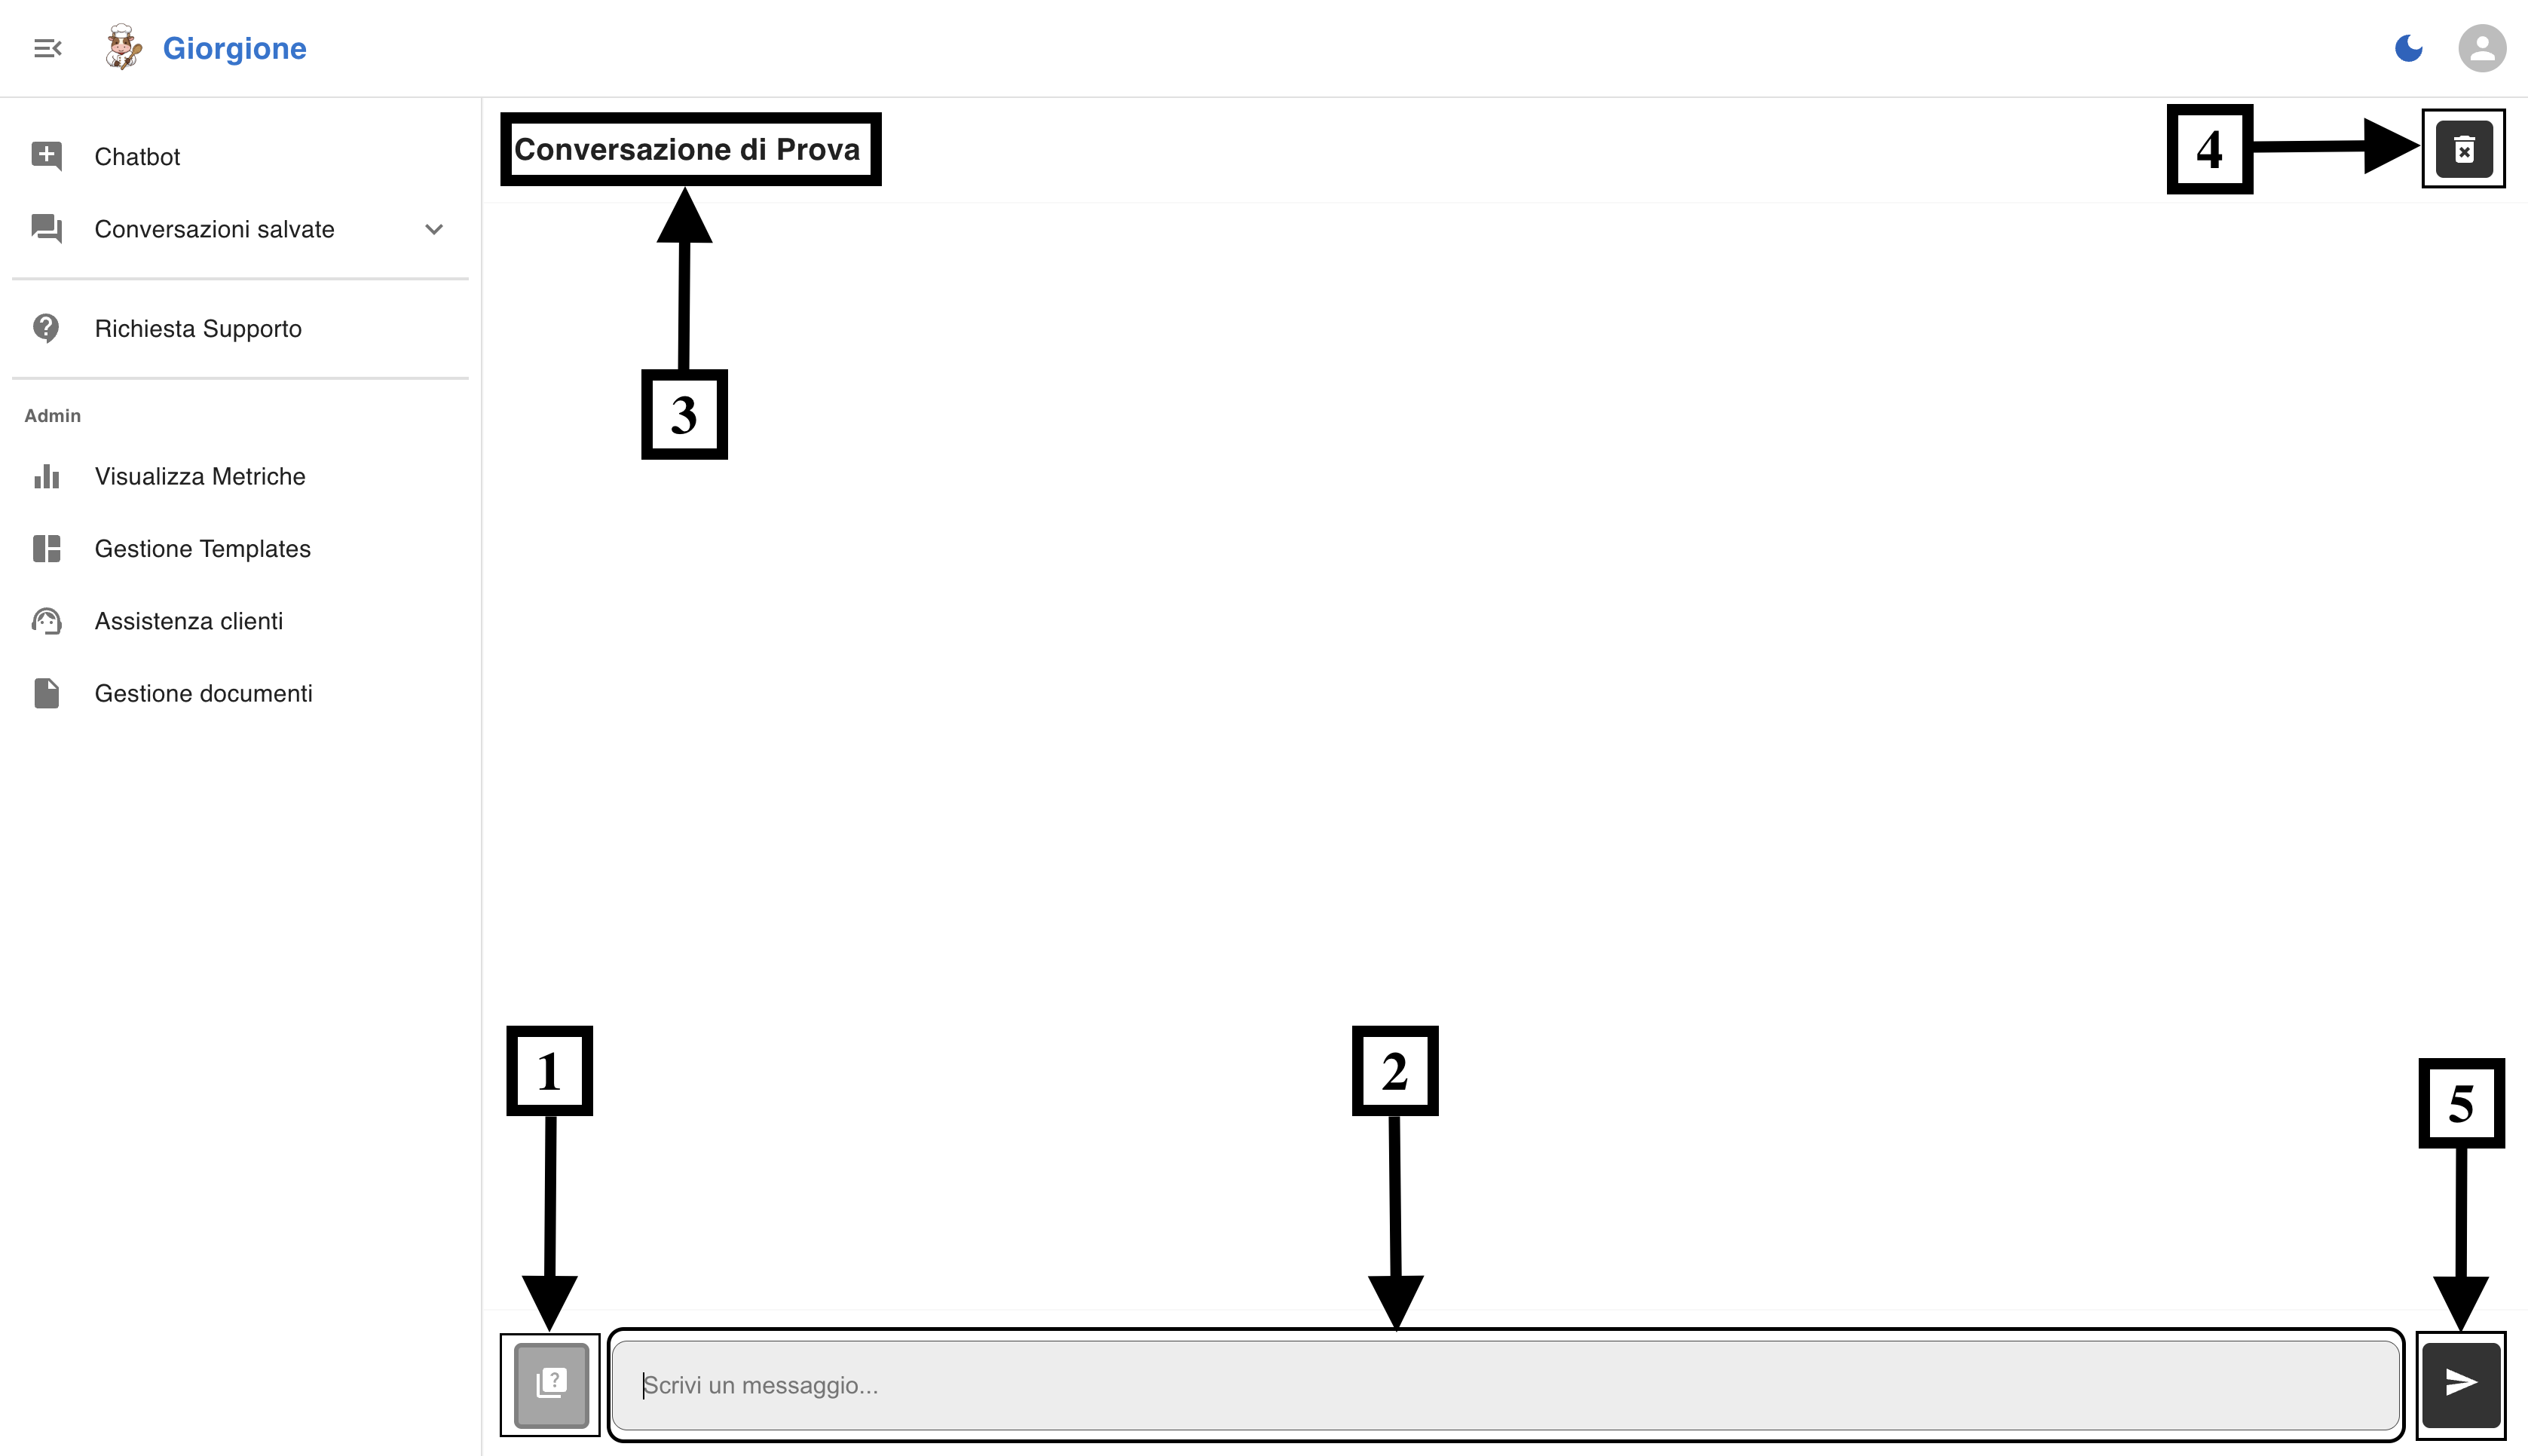
\includegraphics[width=\textwidth]{./img/SchermataChat1.png}
    \caption{Schermata della chat}
    \label{fig:schermata-chat}
\end{figure}
\\
Facendo riferimento alla figura~\ref{fig:schermata-chat} infatti l'utente troverà un bottone per selezionare una domanda templetizzata (\textit{qui segnato con il numero 1}), parleremo di queste più avanti.
Il punto numero 2 indica invece la casella di testo dove l'utente potrà scrivere il proprio messaggio da inviare al bot.
Il punto numero 3 indica il nome della conversazione precedentemente scelto nella schermata iniziale. Il punto numero 4 indica un bottone che permette di eliminare la chat premendolo apparirà un pop-up che chiede cortesemente all'utente se è sicuro di voler eliminare la conversazione figura~\ref{fig:elimina-chat}:
\begin{figure}[h!]
    \centering
    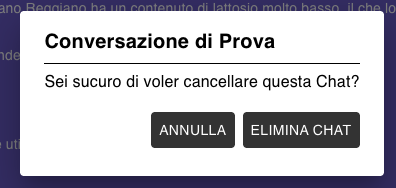
\includegraphics[width=0.5\textwidth]{./img/eliminaChat.png}
    \caption{Elimina chat}
    \label{fig:elimina-chat}
\end{figure}
\\
Il punto numero 5 in figura~\ref{fig:schermata-chat} è il pulsante invio che permette di mandare un messaggio al nostro assistente virtuale. Bisogna dire tuttavia che è possibile inviare un messaggio solo se del testo è presente nella casella di testo (\textit{punto 2 in figura~\ref{fig:schermata-chat}}) e che non è necessario cliccare sul pulsante in quanto è possibile premere direttamente invio sulla tastiera.
\\
Inviato un messaggio questo apparirà nella parte destra della schermata come avviene nelle più famose chat di messaggistica (fare riferimento a figura~\ref{fig:Elaborazione} punto 6), e verrà mostrato il messaggio e la data e l'ora dell'invio.
Nella parte sinistra l'utente potrà osservare il nostro Assistente virtuale Giorgione elaborare il messaggio per soddisfare la richiesta dell'utente (punto 7 figura~\ref{fig:Elaborazione}).
\begin{figure}[h!]
    \centering
    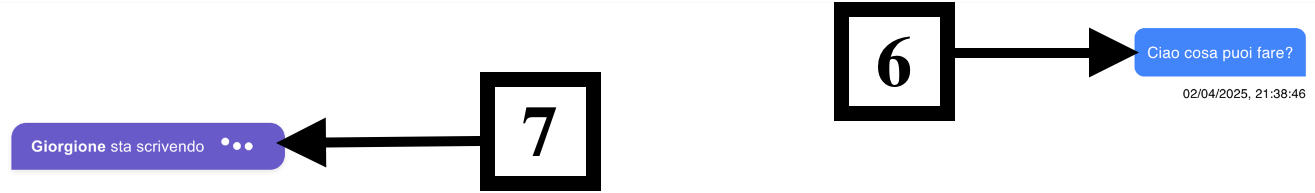
\includegraphics[width=\textwidth]{./img/SchermataChat2.png}
    \caption{Elaborazione del messaggio}
    \label{fig:Elaborazione}
\end{figure}
\\
Una volta mandato il messaggio esso sarà visualizzabile come mostrato in figura~\ref{fig:Visualizzazione Risposta} punto 8, e l'utente potrà decidere opzionalmente se è soddisfatto della risposta data dal bot di fornire una valutazione booleana indicata da un pollice in su e pollice in giù (\textit{figura~\ref{fig:Visualizzazione Risposta} punto 9}):
\begin{figure}[h!]
    \centering
    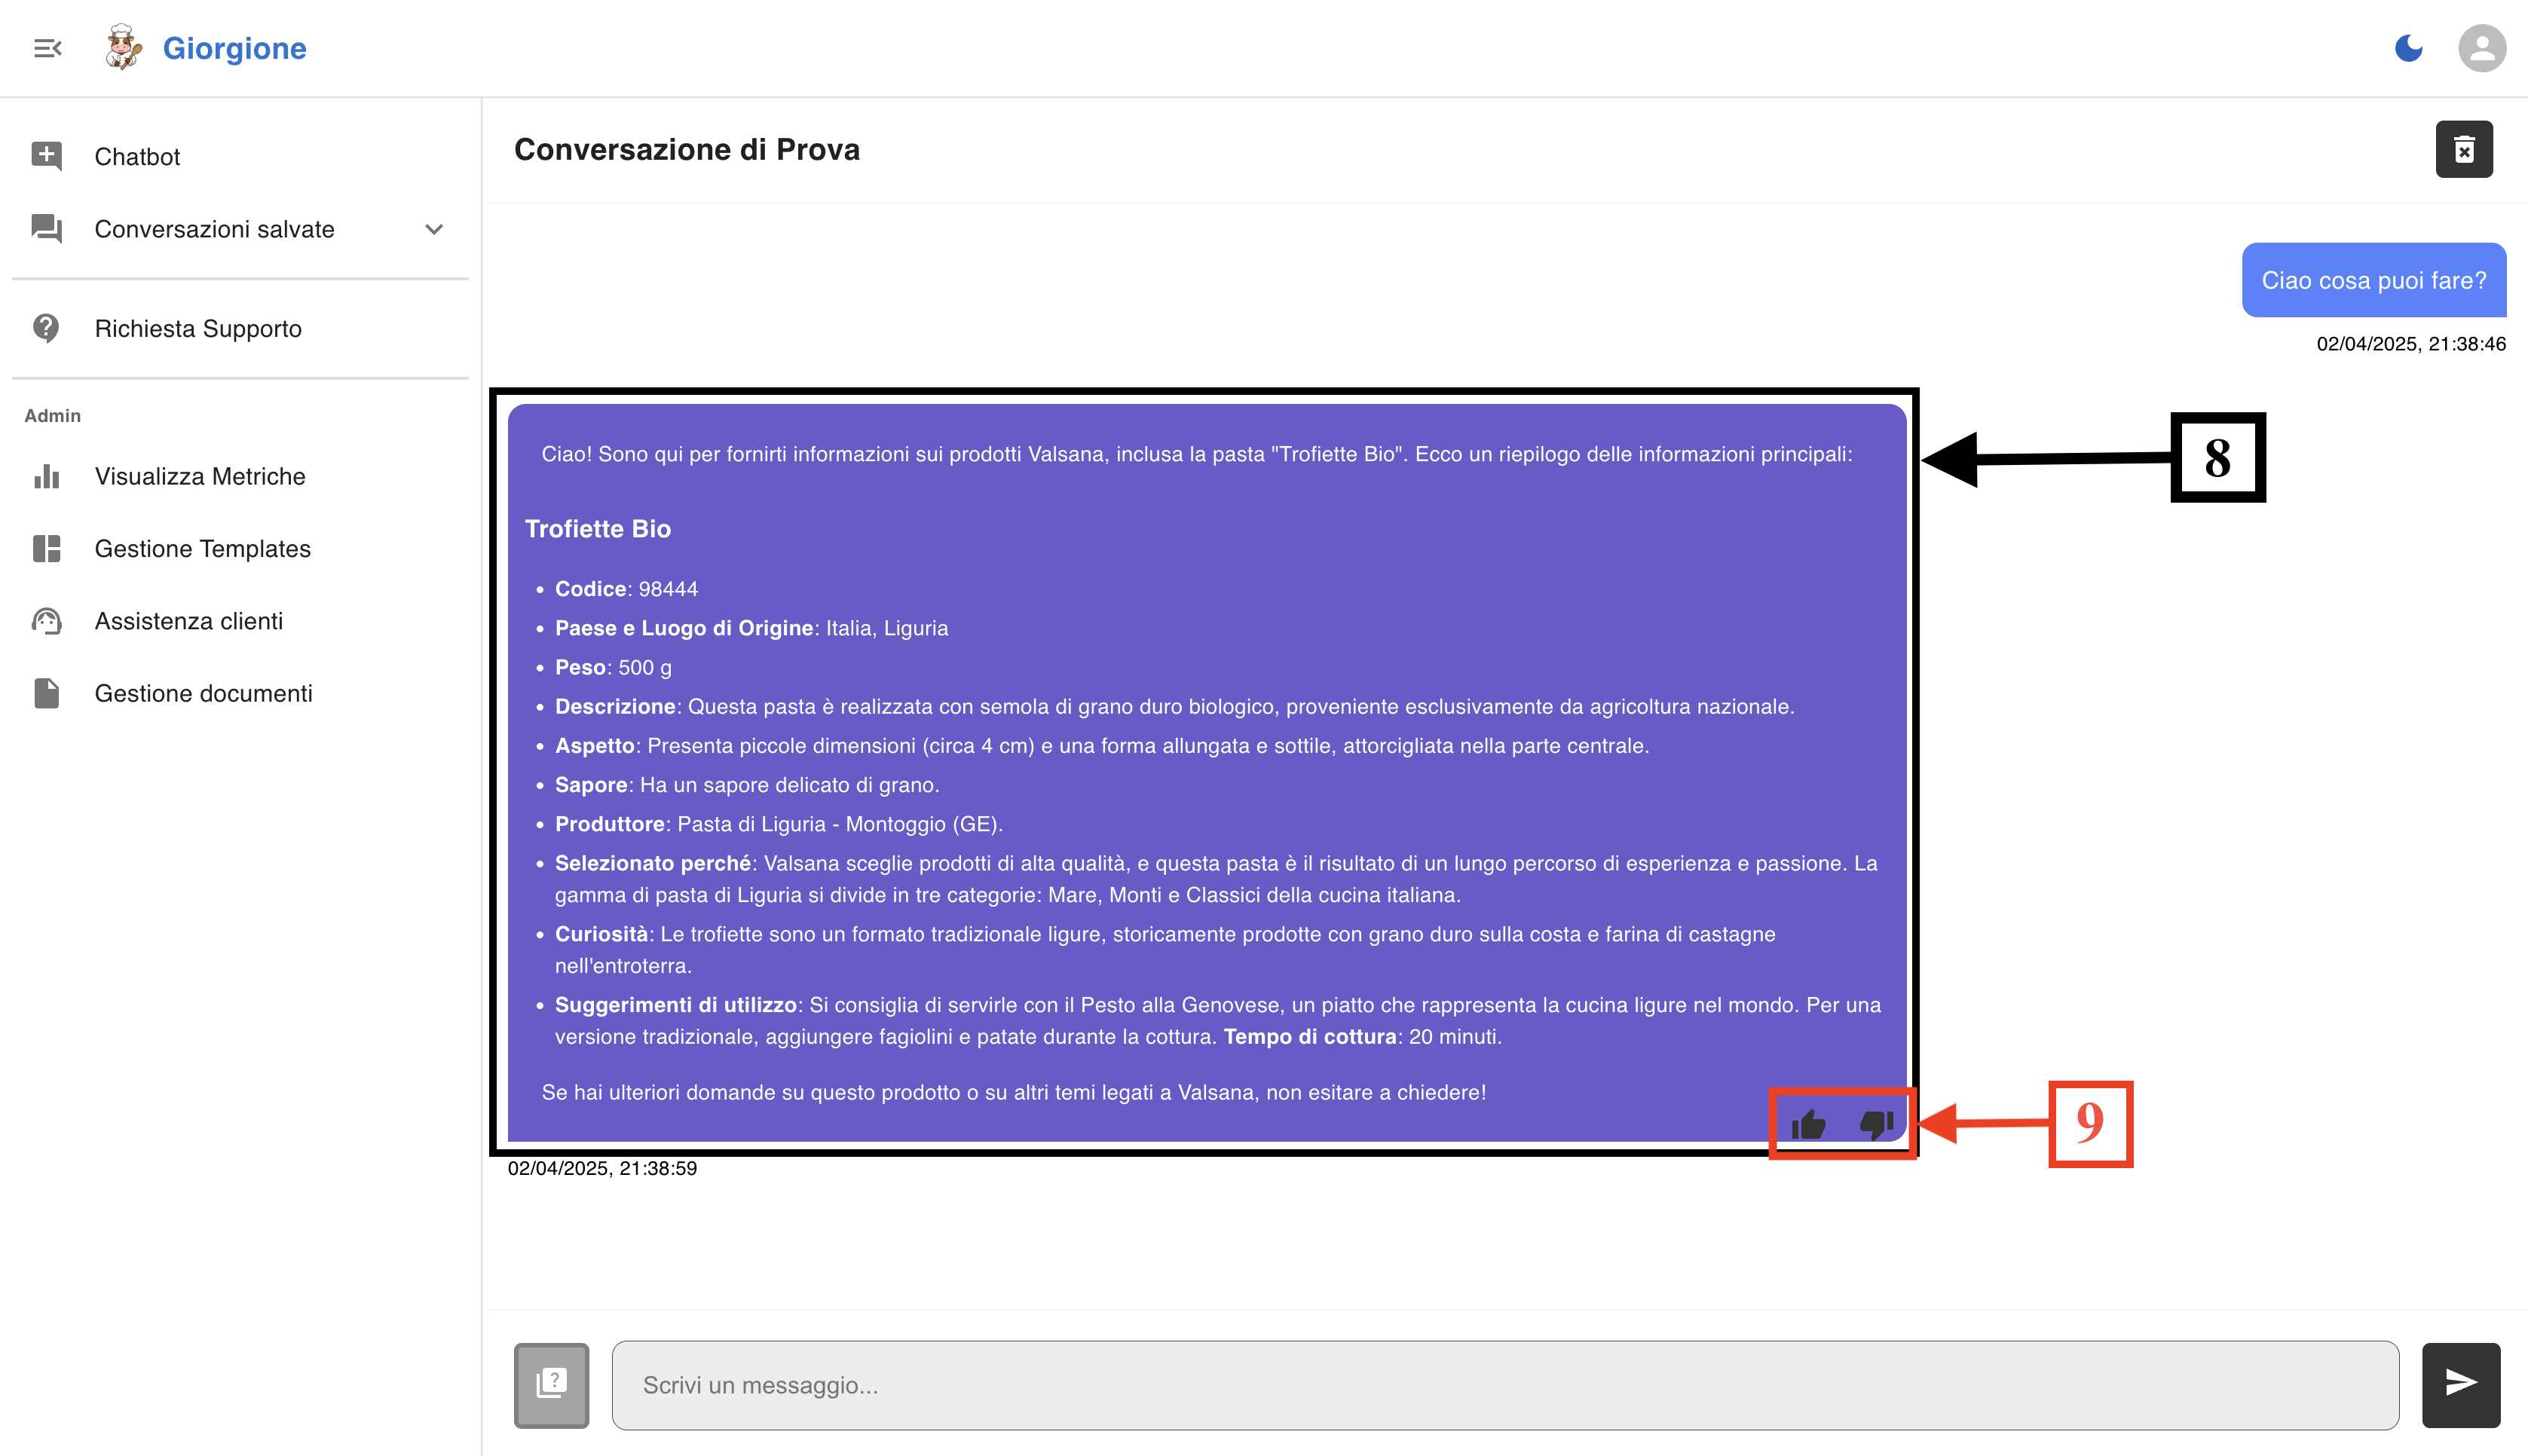
\includegraphics[width=\textwidth]{./img/SchermataChat3.png}
    \caption{Visualizzazione Risposta}
    \label{fig:Visualizzazione Risposta}
\end{figure}
L'utente è notificato dalla scelta dall'illuminazione di uno dei 2 bottoni come mostrato in figura~\ref{fig:likedislike}
\begin{figure}[h!]
    \centering
    \begin{subfigure}{0.2\textwidth}
        \centering
        
\includegraphics[width=\textwidth]{./img/like.png}
        \caption{Caso in cui l'utente scelga like}
    \end{subfigure}
    \hspace{0.05\textwidth}
    \begin{subfigure}{0.2\textwidth}
        \centering
        
\includegraphics[width=\textwidth]{./img/dislike.png}
        \caption{Caso in cui l'utente scelga dislike}
    \end{subfigure}
    \caption{Feedback Risposta}
    \label{fig:likedislike}
\end{figure}